\begin{figure}[h]
	\centering
	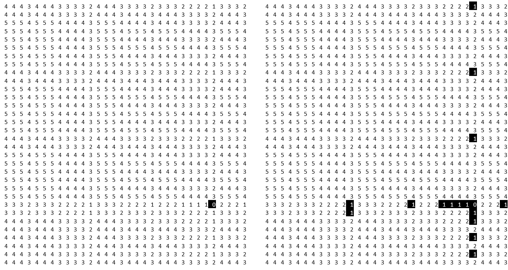
\includegraphics[width=2.5in]{contents/00_images/0-1}\vspace*{5pt}
	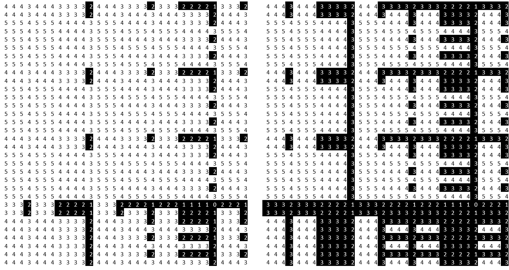
\includegraphics[width=2.5in]{contents/00_images/2-3}\vspace*{5pt}
	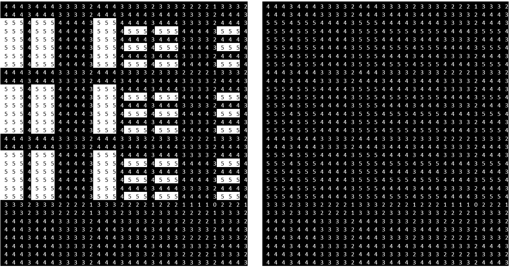
\includegraphics[width=2.5in]{contents/00_images/4-5}
	
	\caption{Bit patterns followed by blocks of size $4^{5}=32\times32$ in the bit-based representation of $\mathcal{N}(\texttt{acgtacgtacgt},5)$. Black signifies a 1. There are $(5+2)=7$ possible patterns---the empty pattern (all 0s) is not shown. Images from \cite{sia2015}}
	\label{fig:bit_patterns}
\end{figure}